\documentclass[10pt, compress]{beamer}

\usetheme{m}

\usepackage{booktabs}
\usepackage{xcolor}
\usepackage[scale=2]{ccicons}
\usepackage{listings}
\usepackage{graphicx}

\usepgfplotslibrary{dateplot}
\setcounter{tocdepth}{1}

%Colors
\definecolor{light_gray}{HTML}{aaaaaa}

%Commands
\newcommand{\up}[1]{\textsuperscript{\textbf{\textsc{#1}}}}
%\setbeameroption{show notes}
\lstset{language=Java,
                columns=flexible,
  basicstyle={\tiny\ttfamily},
  numberstyle=\tiny\color{gray},
  keywordstyle=\color{orange},
  commentstyle=\color{light_gray},
  stringstyle=\color{orange},
  tabsize=2,
  aboveskip=5pt,
  belowskip=5pt,
}

\title{Conception et développement d’une application d’annotation thématique}
\subtitle{dans l’environnement Gate}
\date{}
\author{Charles Follet \and Roland Bary}
\institute{Université de Pau et Pays de l'Adour}

\begin{document}
\maketitle
%%%%% Introduction %%%%%%%%%
\begin{frame}[fragile]
	\frametitle{Introduction}
		\begin{itemize}[<+->]
  			\setbeamertemplate{itemize item}[square]
  			\item{Annotation sémantique : phase en amont de la recherche d'information sémantique}
  			\item{Utilisation de la plate-forme GATE Developper}
  			\item{Problématique : comment annoter de manière automatique un document texte non-structuré ?}		
  		\end{itemize}
\end{frame}
%%%% Sommaire %%%%%%%%%%
\begin{frame}[fragile]
  \frametitle{Sommaire}
  \tableofcontents
\end{frame}
%%%%%% Comprehension du domaine %%%%%%%
\section{Compréhension du domaine}
\begin{frame}[fragile]
	\frametitle{Compréhension du domaine - La ressource}
	\onslide<1->{
	Recherches sur le Numéraire Carolingien de Georges DEPEYROT.\\~\\
	\begin{columns}
		\column{.4\linewidth}
			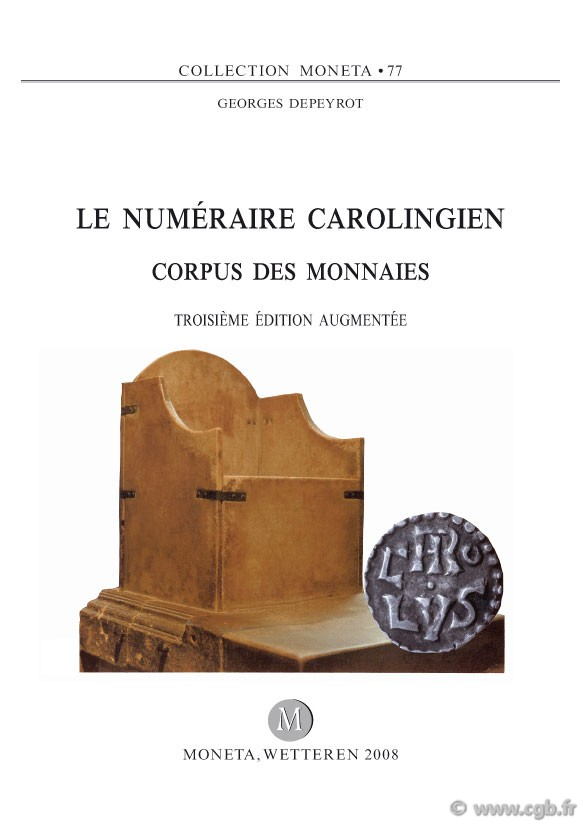
\includegraphics[scale=0.2]{img/depeyrot.jpg}
		\column{.6\linewidth}
		Pouvoir répondre aux questions suivantes:
		\begin{scriptsize}
			\begin{itemize}
				\setbeamertemplate{itemize item}[square]
				\item{Temporelles : Quelles étaient les pièces en circulation de l’an 859 à l’an 865 ?}
				\item{Thématiques : Combien d’exemplaires de la monnaie d’or de Charles le Chauve ont été étudiés ?\\
				Dans quels ateliers, les pièces de type Obole de Charlemagne ont été produites ?}
			\end{itemize}	
		\end{scriptsize}
	\end{columns}
	}
\end{frame}
%%%%%%%%%%%%%%%%%%%%%%%%%%%%%%%%%%%%%%%%%%%%%%%%%%%%%%%%%%%%%%%
\begin{frame}[fragile]
	\frametitle{Compréhension du domaine - l'OCRisation}
	\begin{center}
	Etape d'OCRisation du numéraire.\\~\\
	
\includegraphics[scale=.4]{img/ocr.png} 
	\end{center}
\end{frame}
%%%%%%%%%%%%%%%%%%%%%%%%%%%%%%%%%%%%%%%%%%%%%%%%%%%%
\begin{frame}[fragile]
\frametitle{Compréhension du domaine - Structure du numéraire}
\begin{scriptsize}
Agen (Lot-et-Garonne)\\~\\

Type de 793/4-812: Charlemagne (768-814)\\
Denier de Charlemagne (24 exemplaires étudiés)\\
+ CARLVS REX FR croix~~~~~~~ + AGINNO monogramme\\
Gariel XXII 26; Morrison-Grunthal 177-179; Depeyrot (1) (2) 1; Collections: Berlin 1,64, 1,45;\\
Bruxelles 1,25, 1,25; Charleville-Mézières 1,56; Copenhague 1,31; Garett 1,73; Grenoble; MEC 735 \\
(1,57), 736 (1,24); Monnaie de Paris 88 (1,55); New York 1,64, 1,57; Prou 792 (1,36), 793 (1,60), \\
794 (1,50) Trésors: Biebrich (790-814), 2 ex. (MG 11, Vôlkers, p. 182) (1,60); Ibersheim (814), 1 ex. \\
(MG 13, Vôlkers, p. 186) (1,64); Dorestad (822), 4 ex. (MG 18, Vôlkers, p. 139; H. 7) (1,35);\\
Trouvailles: Bolsward, 1 ex. (H. 528) (1,26).
\end{scriptsize}
\note{Le Numeraire est organisé en atelier, un atelier fabrique une ou plusieurs monnaies. On voit ici l'atelier d'Agen. Nous allons détailler tous les éléments à l'écran}
\end{frame}

\begin{frame}[fragile]
  \frametitle{Compréhension du domaine - L'atelier}
  \begin{scriptsize}
\textbf{Agen (Lot-et-Garonne)}\\~\\
\textcolor{light_gray}{
Type de 793/4-812: Charlemagne (768-814)\\
Denier de Charlemagne (24 exemplaires étudiés)\\
+ CARLVS REX FR croix~~~~~~~ + AGINNO monogramme\\
Gariel XXII 26; Morrison-Grunthal 177-179; Depeyrot (1) (2) 1; Collections: Berlin 1,64, 1,45; \\
Bruxelles 1,25, 1,25; Charleville-Mézières 1,56; Copenhague 1,31; Garett 1,73; Grenoble; MEC 735 \\
(1,57), 736 (1,24); Monnaie de Paris 88 (1,55); New York 1,64, 1,57; Prou 792 (1,36), 793 (1,60), \\
794 (1,50) Trésors: Biebrich (790-814), 2 ex. (MG 11, Vôlkers, p. 182) (1,60); Ibersheim (814), 1 ex. \\
(MG 13, Vôlkers, p. 186) (1,64); Dorestad (822), 4 ex. (MG 18, Vôlkers, p. 139; H. 7) (1,35); \\Trouvailles: Bolsward, 1 ex. (H. 528) (1,26).
} 
\end{scriptsize}
    
    \note{Forme : Ville (Dpt|Pays)?}
\end{frame}

\begin{frame}[fragile]
  \frametitle{Compréhension du domaine - Le type}
  \begin{scriptsize}
\textcolor{light_gray}{Agen (Lot-et-Garonne)}\\~\\

\textbf{Type de 793/4-812: Charlemagne (768-814)}\\
\textcolor{light_gray}{
Denier de Charlemagne (24 exemplaires étudiés)\\
+ CARLVS REX FR croix~~~~~~~ + AGINNO monogramme\\
Gariel XXII 26; Morrison-Grunthal 177-179; Depeyrot (1) (2) 1; Collections: Berlin 1,64, 1,45; \\
Bruxelles 1,25, 1,25; Charleville-Mézières 1,56; Copenhague 1,31; Garett 1,73; Grenoble; MEC 735 \\
(1,57), 736 (1,24); Monnaie de Paris 88 (1,55); New York 1,64, 1,57; Prou 792 (1,36), 793 (1,60), \\
794 (1,50) Trésors: Biebrich (790-814), 2 ex. (MG 11, Vôlkers, p. 182) (1,60); Ibersheim (814), 1 ex. \\
(MG 13, Vôlkers, p. 186) (1,64); Dorestad (822), 4 ex. (MG 18, Vôlkers, p. 139; H. 7) (1,35); \\Trouvailles: Bolsward, 1 ex. (H. 528) (1,26).
} 
    \end{scriptsize}
    
    \note{Forme : Perdiode(souverains)+}
\end{frame}

\begin{frame}[fragile]
  \frametitle{Compréhension du domaine - La nature}
  \begin{scriptsize}
\textcolor{light_gray}{Agen (Lot-et-Garonne)}\\~\\

\textcolor{light_gray}{Type de 793/4-812: Charlemagne (768-814)}\\

\textbf{Denier de Charlemagne (24 exemplaires étudiés)}\\
\textcolor{light_gray}{
+ CARLVS REX FR croix~~~~~~~ + AGINNO monogramme\\
Gariel XXII 26; Morrison-Grunthal 177-179; Depeyrot (1) (2) 1; Collections: Berlin 1,64, 1,45; \\
Bruxelles 1,25, 1,25; Charleville-Mézières 1,56; Copenhague 1,31; Garett 1,73; Grenoble; MEC 735 \\
(1,57), 736 (1,24); Monnaie de Paris 88 (1,55); New York 1,64, 1,57; Prou 792 (1,36), 793 (1,60), \\
794 (1,50) Trésors: Biebrich (790-814), 2 ex. (MG 11, Vôlkers, p. 182) (1,60); Ibersheim (814), 1 ex. \\
(MG 13, Vôlkers, p. 186) (1,64); Dorestad (822), 4 ex. (MG 18, Vôlkers, p. 139; H. 7) (1,35); \\Trouvailles: Bolsward, 1 ex. (H. 528) (1,26).
} 
    \end{scriptsize}
        \note{Forme : Denier, Obole, ... + NOM SOUVERAIN}
\end{frame}

\begin{frame}[fragile]
  \frametitle{Compréhension du domaine - La légende}
  \begin{scriptsize}
\textcolor{light_gray}{Agen (Lot-et-Garonne)}\\~\\

\textcolor{light_gray}{Type de 793/4-812: Charlemagne (768-814)\\
Denier de Charlemagne (24 exemplaires étudiés)}\\

\textbf{+ CARLVS REX FR croix~~~~~~~ + AGINNO monogramme}\\
\textcolor{light_gray}{
Gariel XXII 26; Morrison-Grunthal 177-179; Depeyrot (1) (2) 1; Collections: Berlin 1,64, 1,45; \\
Bruxelles 1,25, 1,25; Charleville-Mézières 1,56; Copenhague 1,31; Garett 1,73; Grenoble; MEC 735 \\
(1,57), 736 (1,24); Monnaie de Paris 88 (1,55); New York 1,64, 1,57; Prou 792 (1,36), 793 (1,60), \\
794 (1,50) Trésors: Biebrich (790-814), 2 ex. (MG 11, Vôlkers, p. 182) (1,60); Ibersheim (814), 1 ex. \\
(MG 13, Vôlkers, p. 186) (1,64); Dorestad (822), 4 ex. (MG 18, Vôlkers, p. 139; H. 7) (1,35); \\
Trouvailles: Bolsward, 1 ex. (H. 528) (1,26).
} 
    \end{scriptsize}
        \note{Forme :+?LEG droit SPACE  +?LEG revers}
\end{frame}

\begin{frame}[fragile]
  \frametitle{Compréhension du domaine - Les collections}
  \begin{scriptsize}
\textcolor{light_gray}{Agen (Lot-et-Garonne)}\\~\\

\textcolor{light_gray}{
Type de 793/4-812: Charlemagne (768-814)\\
Denier de Charlemagne (24 exemplaires étudiés)\\
+ CARLVS REX FR croix~~~~~~~ + AGINNO monogramme
}\\
\textcolor{light_gray}{
Gariel XXII 26; Morrison-Grunthal 177-179; Depeyrot (1) (2) 1; }\textbf{Collections: Berlin 1,64, 1,45; \\
Bruxelles 1,25, 1,25; Charleville-Mézières 1,56; Copenhague 1,31; Garett 1,73; Grenoble; MEC 735 \\
(1,57), 736 (1,24); Monnaie de Paris 88 (1,55); New York 1,64, 1,57; Prou 792 (1,36), 793 (1,60), \\
794 (1,50) }\textcolor{light_gray}{Trésors: Biebrich (790-814), 2 ex. (MG 11, Vôlkers, p. 182) (1,60); Ibersheim (814), 1 ex. \\(MG 13, Vôlkers, p. 186) (1,64); Dorestad (822), 4 ex. (MG 18, Vôlkers, p. 139; H. 7) (1,35); \\Trouvailles: Bolsward, 1 ex. (H. 528) (1,26).
} 
    \end{scriptsize}
\end{frame}

\begin{frame}[fragile]
  \frametitle{Compréhension du domaine - Les trésors}
  \begin{scriptsize}
\textcolor{light_gray}{Agen (Lot-et-Garonne)}\\~\\

\textcolor{light_gray}{
Type de 793/4-812: Charlemagne (768-814)\\
Denier de Charlemagne (24 exemplaires étudiés)\\
+ CARLVS REX FR croix~~~~~~~ + AGINNO monogramme
}\\
\textcolor{light_gray}{
Gariel XXII 26; Morrison-Grunthal 177-179; Depeyrot (1) (2) 1;
Collections: Berlin 1,64, 1,45; \\
Bruxelles 1,25, 1,25; Charleville-Mézières 1,56; Copenhague 1,31; Garett 1,73; Grenoble; MEC 735 \\
(1,57), 736 (1,24); Monnaie de Paris 88 (1,55); New York 1,64, 1,57; Prou 792 (1,36), 793 (1,60), \\
794 (1,50) }\textbf{Trésors: Biebrich (790-814), 2 ex. (MG 11, Vôlkers, p. 182) (1,60); Ibersheim (814), 1 ex. \\
(MG 13, Vôlkers, p. 186) (1,64); Dorestad (822), 4 ex. (MG 18, Vôlkers, p. 139; H. 7) (1,35); }\\
\textcolor{light_gray}{
Trouvailles: Bolsward, 1 ex. (H. 528) (1,26).
} 
    \end{scriptsize}
\end{frame}

\begin{frame}[fragile]
  \frametitle{Compréhension du domaine - Les trouvailles}
  \begin{scriptsize}
\textcolor{light_gray}{Agen (Lot-et-Garonne)}\\~\\

\textcolor{light_gray}{
Type de 793/4-812: Charlemagne (768-814)\\
Denier de Charlemagne (24 exemplaires étudiés)\\
+ CARLVS REX FR croix~~~~~~~ + AGINNO monogramme
}\\
\textcolor{light_gray}{
Gariel XXII 26; Morrison-Grunthal 177-179; Depeyrot (1) (2) 1;
Collections: Berlin 1,64, 1,45; \\
Bruxelles 1,25, 1,25; Charleville-Mézières 1,56; Copenhague 1,31; Garett 1,73; Grenoble; MEC 735 \\
(1,57), 736 (1,24); Monnaie de Paris 88 (1,55); New York 1,64, 1,57; Prou 792 (1,36), 793 (1,60), \\
794 (1,50) Trésors: Biebrich (790-814), 2 ex. (MG 11, Vôlkers, p. 182) (1,60); Ibersheim (814), 1 ex. \\
(MG 13, Vôlkers, p. 186) (1,64); Dorestad (822), 4 ex. (MG 18, Vôlkers, p. 139; H. 7) (1,35); }\\
\textbf{Trouvailles: Bolsward, 1 ex. (H. 528) (1,26).}
    \end{scriptsize}
\end{frame}
%%%%%%%%%%%%%%%%%%%%%%%%%%%%%%%%%%%%%%%%%%%%%%%%%%%%%%%%%%
\begin{frame}[fragile]
	\frametitle{Compréhension du domaine - Scénario d'annotation}

	\textbf{Texte en entrée de notre chaîne de traitement}\\~\\~\\
\begin{scriptsize}
Agen (Lot-et-Garonne)\\~\\

Type de 793/4-812: Charlemagne (768-814)\\
Denier de Charlemagne (24 exemplaires étudiés)\\
+ CARLVS REX FR croix~~~~~~~ + AGINNO monogramme\\
Gariel XXII 26; Morrison-Grunthal 177-179; Depeyrot (1) (2) 1; Collections: Berlin 1,64, 1,45;\\
Bruxelles 1,25, 1,25; Charleville-Mézières 1,56; Copenhague 1,31; Garett 1,73; Grenoble; MEC 735 \\
(1,57), 736 (1,24); Monnaie de Paris 88 (1,55); New York 1,64, 1,57; Prou 792 (1,36), 793 (1,60), \\
794 (1,50) Trésors: Biebrich (790-814), 2 ex. (MG 11, Vôlkers, p. 182) (1,60); Ibersheim (814), 1 ex. \\
(MG 13, Vôlkers, p. 186) (1,64); Dorestad (822), 4 ex. (MG 18, Vôlkers, p. 139; H. 7) (1,35);\\
Trouvailles: Bolsward, 1 ex. (H. 528) (1,26).
\end{scriptsize}

\end{frame}

\begin{frame}[fragile]
	\frametitle{Compréhension du domaine - Scénario d'annotation}

	\textbf{Texte en sortie de notre chaîne de traitement}\\
	Domaine annoté : \colorbox{red!30}{Temporel}.\\~\\~\\
\begin{scriptsize}
Agen (Lot-et-Garonne)\\~\\

Type de \colorbox{red!30}{793/4-812}: Charlemagne (\colorbox{red!30}{768-814})\\
Denier de Charlemagne (24 exemplaires étudiés)\\
+ CARLVS REX FR croix~~~~~~~ + AGINNO monogramme\\
Gariel XXII 26; Morrison-Grunthal 177-179; Depeyrot (1) (2) 1; Collections: Berlin 1,64, 1,45;\\
Bruxelles 1,25, 1,25; Charleville-Mézières 1,56; Copenhague 1,31; Garett 1,73; Grenoble; MEC 735 \\
(1,57), 736 (1,24); Monnaie de Paris 88 (1,55); New York 1,64, 1,57; Prou 792 (1,36), 793 (1,60), \\
794 (1,50) Trésors: Biebrich (790-814), 2 ex. (MG 11, Vôlkers, p. 182) (1,60); Ibersheim (814), 1 ex. \\
(MG 13, Vôlkers, p. 186) (1,64); Dorestad (822), 4 ex. (MG 18, Vôlkers, p. 139; H. 7) (1,35);\\
Trouvailles: Bolsward, 1 ex. (H. 528) (1,26).
\end{scriptsize}
\end{frame}

\begin{frame}[fragile]
	\frametitle{Compréhension du domaine}

	\textbf{Texte en sortie de notre chaîne de traitement}\\
	Domaine annoté : \colorbox{blue!30}{Thématique}.\\~\\~\\
\begin{scriptsize}
\colorbox{blue!30}{Agen (Lot-et-Garonne)}\\~\\

\colorbox{blue!30}{Type de 793/4-812}: Charlemagne (768-814)\\
\colorbox{blue!30}{Denier de Charlemagne} (24 exemplaires étudiés)\\
\colorbox{blue!30}{+ CARLVS REX FR croix~~~~~~~ + AGINNO monogramme}\\
Gariel XXII 26; Morrison-Grunthal 177-179; Depeyrot (1) (2) 1; Collections: \colorbox{blue!30}{Berlin 1,64, 1,45;}\\
\colorbox{blue!30}{Bruxelles 1,25, 1,25; Charleville-Mézières 1,56; Copenhague 1,31; Garett 1,73; Grenoble; MEC 735} \\
\colorbox{blue!30}{(1,57), 736 (1,24); Monnaie de Paris 88 (1,55); New York 1,64, 1,57; Prou 792 (1,36), 793 (1,60),} \\
\colorbox{blue!30}{794 (1,50)} Trésors: \colorbox{blue!30}{Biebrich (790-814), 2 ex. (MG 11, Vôlkers, p. 182) (1,60); Ibersheim (814), 1 ex.} \\
\colorbox{blue!30}{(MG 13, Vôlkers, p. 186) (1,64); Dorestad (822), 4 ex. (MG 18, Vôlkers, p. 139; H. 7) (1,35);}\\
Trouvailles: \colorbox{blue!30}{Bolsward, 1 ex. (H. 528) (1,26).}
\end{scriptsize}
\end{frame}


%%%%%% Annotations dans GATE Developper %%%%%%%%
\section{Annotations dans GATE}
\begin{frame}[fragile]
\frametitle{Annotations dans GATE}
\begin{columns}
	\onslide<1>
	\column{.6\linewidth}
	\begin{center}
	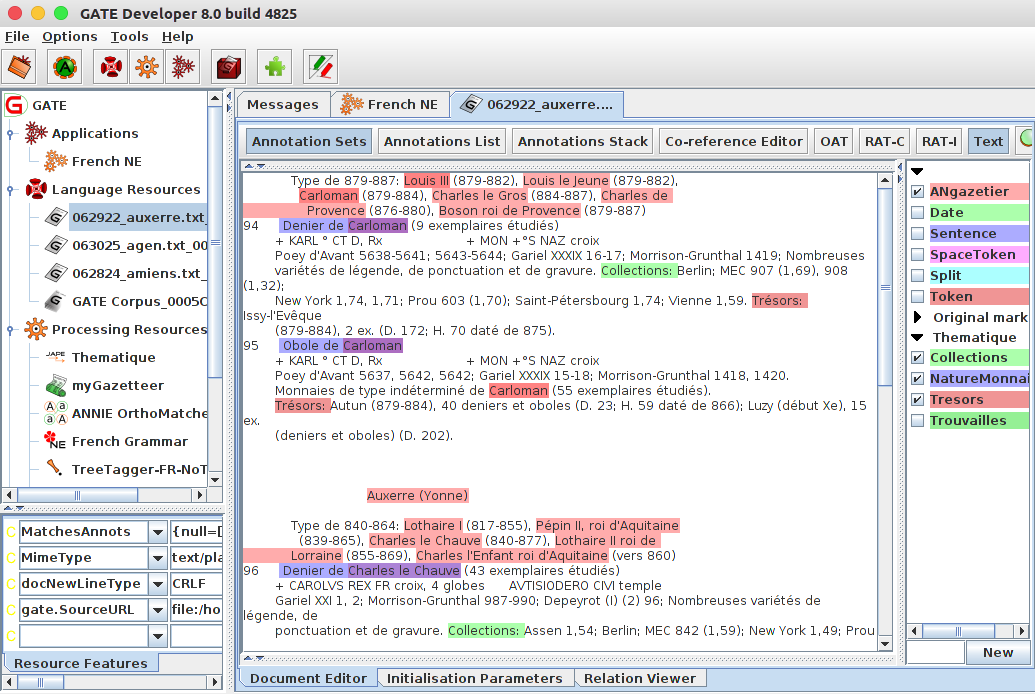
\includegraphics[scale=0.190]{img/gate.png} 
	\end{center}
	\onslide<1>
	\column{.4\linewidth}
	\begin{scriptsize}
		\setbeamertemplate{itemize item}[square]
	\begin{itemize}
		\item{Outil de traitement automatique du langage (en JAVA).}
		\item{Université de Sheffield depuis 1995 (version 8).}
		\item{Principe: Chaîne de traitement (Pipeline).}
		\item{Plusieurs modules dans un pipeline.}
		\item{ANNIE: Pipeline par défaut pouvant servir de chaîne de départ}
	\end{itemize}
	\end{scriptsize}
\end{columns}
\end{frame}

\begin{frame}[fragile]
\frametitle{Annotations dans GATE}
	\begin{center}
	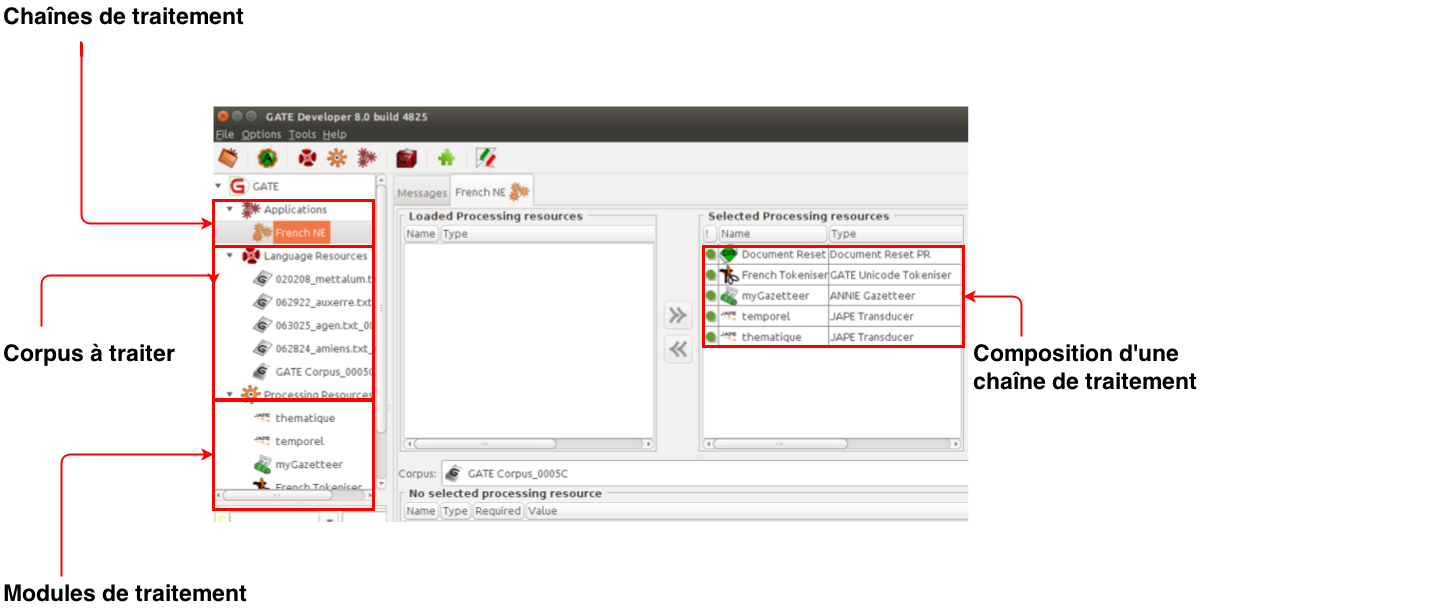
\includegraphics[scale=0.275]{img/gatePresent.png} 
	\end{center}
\end{frame}

\begin{frame}[fragile]
\frametitle{Annotations dans GATE - LANG}
La chaîne de traitement LANG
\begin{center}
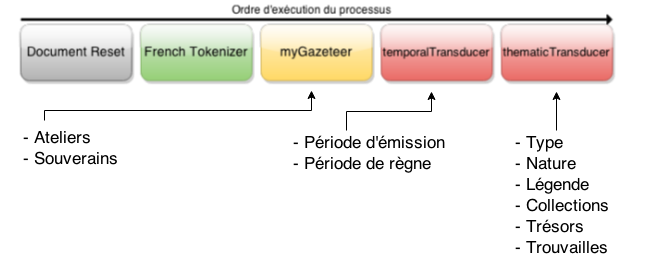
\includegraphics[scale=0.5]{img/chaine1.png} 
\end{center}
\end{frame}

\begin{frame}[fragile]
\frametitle{Annotations dans GATE - LANG}
\begin{center}

\includegraphics[scale=0.5]{img/chaine2.png} 
\end{center}
\begin{itemize}[<+->]
	\setbeamertemplate{itemize item}[square]
	\item{Document reset : Réinitialisation du document}
	\item{French Tokeniser : Découpage des phrases en mots}
	\item{MyGazetter : Identification de noms d'entités par Gazetier}
	\item{temporal/thematic Transducer : Repérage d'entités nommées inconnues en fonction de modèles d'extraction écrits en langage JAPE}
\end{itemize}
\end{frame}

\subsection{Les Gazetiers}
\begin{frame}[fragile]
\frametitle{Annotations dans GATE - Gazetiers}
	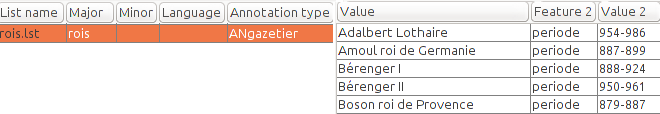
\includegraphics[scale=0.4]{img/gazetier.png} 
		\begin{itemize}[<+->]
			\setbeamertemplate{itemize item}[square]
			\item{liste de noms d'entités (Villes, métiers,etc)}
			\item{permettant un repérage d’occurrences dans un texte}
			\item{possibilité d'associer des caractéristiques a chaque nom d'entité (séparateurs)}
			\item{Dans Gate: MajorType, MinorType réutilisable dans une règle \textit{JAPE}}
		\end{itemize}
\end{frame}

\subsection{Le formalisme JAPE}
\begin{frame}[fragile]
\frametitle{Annotations dans GATE - Le formalisme JAPE}
\begin{columns}
	\onslide<1>
	\column{.6\linewidth}
	\begin{scriptsize}
\begin{lstlisting}
Macro: CHAINE_DEBUT
(
    ({Token.string =="Type"})({SpaceToken})
    ({Token.string =="de"})({SpaceToken})
)

// Exemple : Type de 758/9-762
Rule: PeriodeEmissionRule
/************ Left Hand Side ***********/
(
    CHAINE_DEBUT ({Periode}):p
):PeriodeEmission
/**************************************/
/************ Right Hand Side ***********/
-->:PeriodeEmission.PeriodeEmission = {
 	Kind = "PeriodeEmission" ,
 	D1 = :p.Periode.D1, D2 = :p.Periode.D2
}
/**************************************/
\end{lstlisting}
\end{scriptsize}
	\onslide<1>
	\column{.4\linewidth}
	\begin{scriptsize}
	\begin{itemize}
	\setbeamertemplate{itemize item}[square]
	\item{Règles JAPE en deux blocs}
	\item{Partie gauche (LHS): définition d'un motif d'annotation à repérer}
	\item{Partie droite (RHS): Opérations sur un motif (Code JAVA éventuel)}
	\item{Utilisation d'un système de Macros}
	\end{itemize}
	\end{scriptsize}
\end{columns}
\end{frame}

%%%%%%%%%%%%%%%%%%%%%%%%%%%%%%%%%%%%%
\section{Mise en œuvre}
\begin{frame}[fragile]
  \frametitle{Mise en œuvre - Démarche}
\begin{enumerate}[<+->]
    \item{Langage naturel \onslide<4,5,6>{\hfill \textbf{français}}}
    \item{Langage régulier \onslide<5,6>{\hfill\textbf{expressions régulières}}}
    \item{Langage de programmation \onslide<6>{\hfill\textbf{\textit{JAPE}}}}
\end{enumerate}
\end{frame}

\begin{frame}[fragile]
  \frametitle{Mise en œuvre - Exemple 1}
Annotation : La période d'émission \\
Exemple 1 : \textit{Type de 793/4-812}
\end{frame}

\begin{frame}[fragile,t]
\setbeamercovered{transparent}
  \frametitle{Mise en œuvre - Exemple 1}
\begin{center}
\onslide<2>{Type de} \onslide<1->{793/4-812}
\end{center}
1. \textbf{\textsc{\textbf{Langage naturel}}}\\
\onslide<1->{Une période est un intervalle entre deux dates. Dans notre travail, les dates sont constituées de trois chiffres. En cas d'ambiguïté, une date peut être suivie d'un / et d'un chiffre traduisant l'indétermination de la date.}\\
\onslide<2>{Il faut assurer la capture de la période d'émission en ajoutant la contrainte précédée de "Type de" afin de ne pas récupérer toutes les périodes du document.}
\end{frame}

\begin{frame}[fragile,t]
\setbeamercovered{transparent}
  \frametitle{Mise en œuvre - Exemple 1}
\begin{center}
\onslide<4->{Type de} \onslide<1->{793/4}\onslide<2->{-}\onslide<3->{812}
\end{center}
2. \textbf{\textsc{\textbf{Langage régulier}}}\\
\onslide<4->{Type de : }\onslide<1->{([0-9]\{3\}(/[0-9])?)}\onslide<2->{-}\onslide<3->{([0-9]\{3\}(/[0-9])?)}
\end{frame}

\begin{frame}[fragile,t]
\setbeamercovered{transparent}
  \frametitle{Mise en œuvre - Exemple 1}
\begin{center}
\onslide<1->{Type de} \onslide<2->{793/4}\onslide<2->{-}\onslide<2->{812}
\end{center}
3. \textbf{\textsc{\textbf{Langage de programmation}}}\\
\begin{columns}[t]
  \begin{column}{.5\linewidth}
\onslide<1->
 \begin{lstlisting}
Macro: CHAINE_DEBUT
(
    ({Token.string =="Type"})({SpaceToken})
    ({Token.string =="de"})({SpaceToken})
)
\end{lstlisting}
\onslide<2->
\begin{lstlisting}
Macro: TROIS_NOMBRES
({Token.kind==number,Token.length == 3})
Macro: UN_NOMBRE
({Token.kind==number,Token.length == 1})
Macro:SLASH
({Token.string=="/"})
Macro:DATE_PRECISE
(TROIS_NOMBRES)
Macro:DATE_IMPRECISE
(TROIS_NOMBRES SLASH UN_NOMBRE)
Macro:DATE
(DATE_PRECISE | DATE_IMPRECISE)
\end{lstlisting}
\end{column}


\begin{column}{.5\linewidth}
\onslide<3->
\begin{lstlisting}
Rule: PeriodeRule
((DATE):d1({Token.string =="-"})(DATE):d2)
:Periode -->:Periode{/*...*/}
\end{lstlisting}
\onslide<4->
\begin{lstlisting}
Rule: PeriodeEmissionRule
(CHAINE_DEBUT ({Periode}):p)
:PeriodeEmission
-->:PeriodeEmission.PeriodeEmission = {/*..*/}
\end{lstlisting}
\end{column}
\end{columns}
\end{frame}






\begin{frame}[fragile]
  \frametitle{Mise en œuvre- Exemple 2}
Annotation : La nature de la monnaie \\
Exemple 2 : \textit{Obole de Carloman}
\end{frame}

\begin{frame}[fragile,t]
\setbeamercovered{transparent}
  \frametitle{Mise en œuvre - Exemple 2}
\begin{center}
\onslide<1->{Obole de Carloman}
\end{center}
1. \textbf{\textsc{\textbf{Langage naturel}}}\\
\onslide<1->{La nature de la monnaie est toujours un élément de l'ensemble \{Denier, Obole, Monnaie D'Or, Faux obole, Monnaies de type indéterminé\} suivi du nom d'un souverain. Il suffit donc d'utiliser une expression composée de tous les mots de l'ensemble.}
\end{frame}

\begin{frame}[fragile,t]
\setbeamercovered{transparent}
  \frametitle{Mise en œuvre - Exemple 2}
\begin{center}
\onslide<1->{Obole }\onslide<2->{de }\onslide<3->{Carloman}
\end{center}
2. \textbf{\textsc{\textbf{Langage régulier}}}\\
\begin{scriptsize}
\onslide<1->{[\textbackslash s]\{2,\}(Denier|Obole|Monnaie d'or|Faux Obole|
Monnaies de type indéterminé) }\onslide<2->{(.*) } \onslide<3->{Nom\_Souverain}
\end{scriptsize}

\end{frame}

\begin{frame}[fragile,t]
\setbeamercovered{transparent}
  \frametitle{Mise en œuvre - Exemple 2}
\begin{center}
\onslide<1->{Obole } \onslide<2->{de }\onslide<3->{Carloman}
\end{center}
3. \textbf{\textsc{\textbf{Langage de programmation}}}\\
\begin{columns}[t]
  \begin{column}{.5\linewidth}
\onslide<1->
\begin{lstlisting}
Macro: MONNAIE
(
   ({Token.string == "Obole"})|
   ({Token.string == "Denier"})|
   ({Token.string == "Monnaie d'or"})|
   ({Token.string == "Faux Obole"})|
    ({Token.string == "Monnaies de type indéterminé"})
)
\end{lstlisting}
\onslide<2->
\begin{lstlisting}
Macro: LIAISON
({Token.string == "de"})
\end{lstlisting}
\end{column}


\begin{column}{.5\linewidth}
\onslide<3->
\begin{lstlisting}
Rule: NatureMonnaieRule
(   
   ({SpaceToken})?(MONNAIE):monnaie
   ({SpaceToken})(LIAISON)({SpaceToken})
   ({ANgazetier.majorType == "rois"})
   
):NatureMonnaie 
-->
      :NatureMonnaie.NatureMonnaie = {/* ... */}
\end{lstlisting}
\end{column}
\end{columns}
\end{frame}

\begin{frame}[fragile]
  \frametitle{Mise en œuvre - Résultat}
\textbf{Résultat d'annotation}\\~
Fichier XML : \\
\begin{center}
\alert{$<$PeriodeEmission$>$}Type de 793/4-812\alert{$<$/PeriodeEmission$>$}\\~\\
\alert{$<$NatureMonnaie$>$}Obole de Carloman\alert{$<$/NatureMonnaie$>$}\\~\\
\end{center}
\onslide<2->{\textit{Comment visualiser les annotations en dehors de GATE ?}}\hfill\onslide<3>{\textbf{XSLT}}

\end{frame}
%%%%%% Visualisation %%%%%%%%%
\section{Visualisation}
\begin{frame}[fragile]
  \frametitle{Visualisation}
\begin{center}
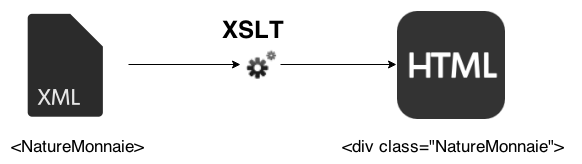
\includegraphics[scale=.5]{img/visualisation.png} 
\end{center}
\end{frame}
%%%% DEMO %%%%%%%%%%%%%%
\section{Démonstration}
%%%%%%% Conclusion %%%%%%%%%%%
\begin{frame}[fragile]
  \frametitle{Conclusion}
\begin{center}
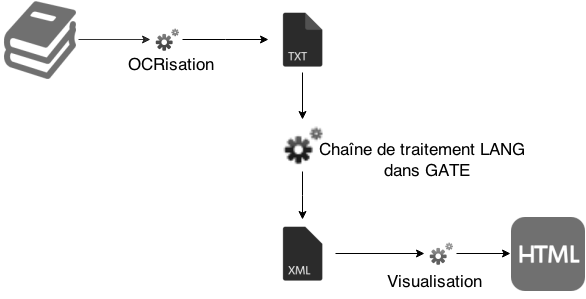
\includegraphics[scale=0.5]{img/conclusion.png}
\end{center}
\end{frame}

\begin{frame}
\frametitle{Conclusion}
\begin{itemize}[<+->]
	\setbeamertemplate{itemize item}[square]
	\item{Amélioration de la robustesse de l'application}
	\item{}
\end{itemize}
\end{frame}
\end{document}